% Chapter Template

\chapter{Optimization on Structures} % Main chapter title
\label{Chapter5} % Change X to a consecutive number; for referencing this chapter elsewhere, use \ref{ChapterX}
\lhead{Chapter 5. \emph{Optimization on Structures}} % Change X to a consecutive number; this is for the header on each page - perhaps a shortened title



\rule{\textwidth}{0.4pt} \\[0.5cm]
\textit{``For the things we have to learn before we can do them, we learn by doing them"}

\begin{flushright}
Aristotle
\end{flushright}
\rule{\textwidth}{0.4pt} 
\newline 
\newline 
This chapter is dedicated to the optimization on structured data. Basically, two forms of structures are considered. First, in section          
\ref{sec:optimize_graph}, optimization on graphical models is studied. Second, in section \ref{sec:optimize_matrix}, structures on 
manifold are considered. More precisely, the optimization on matrix manifolds are studied. 

%----------------------------------------------------------------------------------------
%	SECTION 1
%----------------------------------------------------------------------------------------
\section{Optimization on Graphs}
\label{sec:optimize_graph}
In this section, two optimization methods are reviewed: \emph{max-product (loopy) belief propagation} and \emph{iterated conditional modes} (ICMs).  
Max-product (loopy) belief propagation is an extension of belief propagation inference, which was explained in section \ref{sec:inference}, while 
ICMs is an iterative ``greedy" strategy for local optimization.    
There also exist other notable optimization methods for graphical models, such as \emph{graph cut}, \emph{tree-reweighted message passing}. 
Meanwhile, they are not added in this dissertation. Readers are referred to \cite{many_optimizations} for a review and comparison of them.   



\subsection{Max-product (Loopy) Belief Propagation}
In the belief propagation algorithm (section \ref{sec:inference}), a variable node sends a message to one of its neighbours by first
receiving messages from other neighbours and summing itself out in the product of incoming messages and the occupied potential function.  
Therefore, it is also referred to as \emph{sum-product algorithm} for factor graphs. Optimization actually can be also considered as     
inference by replacing \emph{sum} with \emph{max}, which results in max-product belief propagation, of which the pseudo-code is presented 
in Algorithm \ref{alg:Max_BP_tree}
 \begin{algorithm}
	\caption{Max-product Belief Propagation for tree-structured Markov networks}
	\label{alg:Max_BP_tree}
\begin{algorithmic}[1]
\STATE  select one variable as the root; 
\STATE  starting from all leaves, propagate \emph{beliefs} toward the root as:
\begin{equation*}
m_{i \rightarrow j}(x_j)= \max_{x_i}\left\{\phi(x_i,x_j) \prod_{k\in \text{Ne}(i)\backslash j} m_{k \rightarrow i}(x_i)\right\}
\end{equation*}
\STATE  when the root receives all messages from its neighbors, then propagate backwards the \emph{``inverse beliefs"} as the step 2;
\STATE  the optimization solution of each variable is computed as: 
\begin{equation*}
	x_i=\argmax_{x_i} \prod_{k\in \text{Ne}(i)} m_{k \rightarrow i}(x_i)
\end{equation*}
where Ne$(i)$ denotes the neighboring variables of $x_i$ in the graph. 
\end{algorithmic}
\end{algorithm}

Analogously, the max-product loopy belief propagation can be written out (see Algorithm \ref{alg:max_LBP}) for loopy Markov networks.  
\begin{algorithm}
	\caption{Max-product Loopy Belief Propagation for Loopy Markov networks}
	\label{alg:max_LBP}
\begin{algorithmic}[1]
%\STATE  In a loopy graph, there is no root and leaves because of loop.
\STATE  initialize all messages $m_{i\rightarrow j}$ in both directions of all connected variables randomly or with a constant value (\emph{e.g.} 1);
\WHILE {all messages converge}
\STATE  update messages as:
\begin{equation*}
  m^{(t+1)}_{i \rightarrow j}(x_j)= \max_{x_i}\left\{\phi(x_i,x_j) \prod_{k\in \text{Ne}(i)\backslash j} m^{(t)}_{k \rightarrow i}(x_i)\right\}
\end{equation*}
\ENDWHILE
\end{algorithmic}
\end{algorithm}


\subsection{Iterated Conditional Modes}
Iterated conditional modes (ICMs) is a simple ``greedy" strategy for the optimization of Markov networks. Basically, all variables are initialized randomly and then the state 
of each variable $x_i$ is determined by maximizing the product of all potential functions which involve $x_i$. This state update is iteratively carried out for all variables       
until convergence. 

\section{Optimization on Matrix Manifolds}
\label{sec:optimize_matrix}
In many practical problems, the optimization is with respect to matrices which satisfy certain properties.   
A few examples are enumerated as follow:     
\begin{itemize}
	\item \textbf{Oblique manifold}: $\mathcal{M}=\{X\in\mathbb{R}^{n\times m}: diag (X^\top X)=\mathbf{1}_m \}$; 
	\item \textbf{Stiefel manifold}: $\mathcal{M}=\{X\in\mathbb{R}^{n\times m}: X^\top X=I_m \}$; 
	\item \textbf{SO(n) manifold}: $\mathcal{M}=\{X\in\mathbb{R}^{n\times n}: X^\top X=I_n \text{ and } det(X)=1\}$. 
\end{itemize}
These matrices can also be considered as structures, in which entries are dependent by satisfying different constraints.    
Usually, optimization techniques on matrix manifolds are used to find the optimal matrix. A review of relevant methods      
is provided in \cite{matrix_manifold}.  
In the following subsection, an application of the optimization on the SE(3) manifold on 3D shape registration is presented, which 
shows a representative example of this type of optimization.    

\subsection{3D Point Cloud Registration with Optimization on SE(3) Manifold} 
Despite intensive study, 3D shape
registration remains an open question. 
Here, a novel and efficient registration method is proposed. 
Quite
different from previous registration methods, instead of computing
correspondence and aligning in 3D space, the proposed algorithm first maps 
points to a higher dimensional reproducing  kernel Hilbert space by applying
kernel methods. Registration is subsequently performed within the feature
space by aligning principal components using kernel PCA. The alignment is
projected back into 3D pose space. The whole procedure is
theoretically elegant and efficient. Kernel PCA is used to avoid
explicit computation in feature space, and SE(3) on-manifold
optimization is employed for the convex optimization in the alignment projection. 
Empirical results demonstrate that the proposed method is quite accurate
and robust to various challenging circumstances (\emph{e.g.} large motions,
outliers), and remarkably, it is much faster than other
state-of-the-art methods with comparable performance. 
More technical details and results are presented in the paper IX by the author. 


\begin{shaded}
 {\Huge IX.} \textbf{Hanchen Xiong}, Sandor Szedmak, Justus Piater {\it Efficient, General Point Cloud Registration With Kernel Feature Maps}, 
In Proceedings of 10th International Conference on Computer and Robot Vision (CRV13), pp 83-90, 2013, IEEE.
\end{shaded}
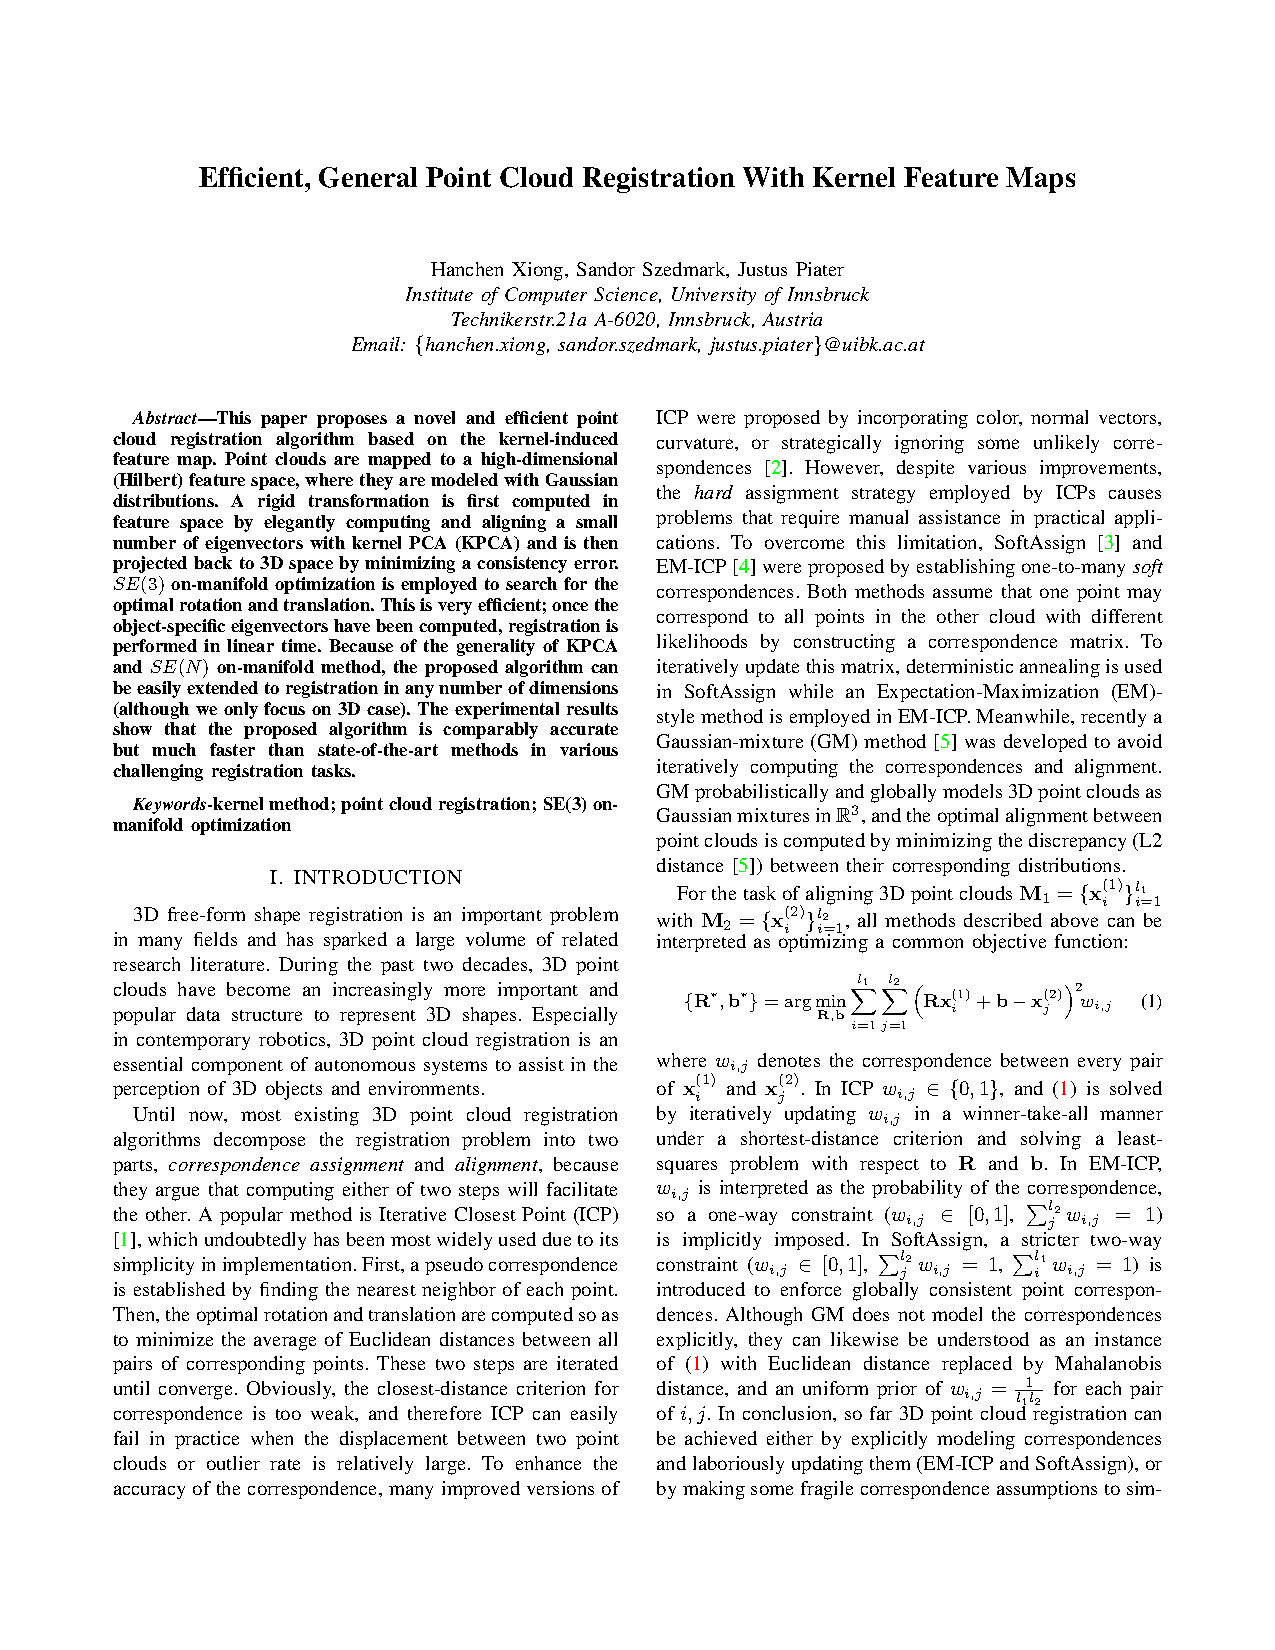
\includepdf[offset=3cm -3cm, scale=1, pages=-,pagecommand={\pagestyle{fancy}}]{./Papers/Xiong-2013-CRV.pdf}


%----------------------------------------------------------------------------------------
%	SECTION 2
%----------------------------------------------------------------------------------------


%\section{Stochastic Optmization of Black-box Functions on Riemannian Manifolds using Kernel Adaptive Sequential Monte Carlo}
%
%Sed ullamcorper quam eu nisl interdum at interdum enim egestas. Aliquam placerat justo sed lectus lobortis ut porta nisl porttitor. Vestibulum mi dolor, lacinia molestie gravida at, tempus vitae ligula. Donec eget quam sapien, in viverra eros. Donec pellentesque justo a massa fringilla non vestibulum metus vestibulum. Vestibulum in orci quis felis tempor lacinia. Vivamus ornare ultrices facilisis. Ut hendrerit volutpat vulputate. Morbi condimentum venenatis augue, id porta ipsum vulputate in. Curabitur luctus tempus justo. Vestibulum risus lectus, adipiscing nec condimentum quis, condimentum nec nisl. Aliquam dictum sagittis velit sed iaculis. Morbi tristique augue sit amet nulla pulvinar id facilisis ligula mollis. Nam elit libero, tincidunt ut aliquam at, molestie in quam. Aenean rhoncus vehicula hendrerit.
%
%
%
